\section{Auswertung}
\label{sec:Auswertung}

\subsection{Kennlinienschar}

In \autoref{tab:kennlinien} sind die Messdaten der fünf Kennlinien aufgetragen.
\begin{table}
  \centering
  \caption{Messwerte der fünf Kennlinien.}
  \label{tab:kennlinien}
  \begin{tabular}{c c c c c c}
    \toprule
    & \multicolumn{1}{c}{$I_{\text{Heiz}} = \qty{2.0}{\ampere}$} &
      \multicolumn{1}{c}{$I_{\text{Heiz}} = \qty{2.1}{\ampere}$} &
      \multicolumn{1}{c}{$I_{\text{Heiz}} = \qty{2.2}{\ampere}$} &
      \multicolumn{1}{c}{$I_{\text{Heiz}} = \qty{2.3}{\ampere}$} &
      \multicolumn{1}{c}{$I_{\text{Heiz}} = \qty{2.4}{\ampere}$} \\
      \cmidrule(lr){2-2}\cmidrule(lr){3-3}\cmidrule(lr){4-4}\cmidrule(lr){5-5}\cmidrule(lr){6-6}

    $U \mathbin{/} \unit{\volt}$ &
    $I \mathbin{/} \unit{\milli\ampere}$ &
    $I \mathbin{/} \unit{\milli\ampere}$ &
    $I \mathbin{/} \unit{\milli\ampere}$ & 
    $I \mathbin{/} \unit{\milli\ampere}$ &
    $I \mathbin{/} \unit{\milli\ampere}$ \\
    \midrule
       0 & 0,000 &   0,000 &   0,000 &   0,000 &   0,000 \\
       5 & 0,010 &   0,012 &   0,014 &   0,016 &   0,017 \\
      10 & 0,022 &   0,028 &   0,033 &   0,036 &   0,039 \\
      15 & 0,034 &   0,045 &   0,053 &   0,058 &   0,061 \\
      20 & 0,044 &   0,062 &   0,076 &   0,084 &   0,089 \\
      25 & 0,060 &   0,080 &   0,096 &   0,104 &   0,110 \\
      30 & 0,070 &   0,096 &   0,116 &   0,130 &   0,137 \\
      35 & 0,082 &   0,114 &   0,140 &   0,158 &   0,169 \\
      40 & 0,092 &   0,134 &   0,168 &   0,194 &   0,207 \\
      45 & 0,102 &   0,155 &   0,201 &   0,230 &   0,246 \\
      50 & 0,107 &   0,170 &   0,228 &   0,265 &   0,287 \\
      60 & 0,111 &   0,213 &   0,285 &   0,337 &   0,371 \\
      70 & 0,119 &   0,231 &   0,340 &   0,425 &   0,480 \\
      80 & 0,123 &   0,247 &   0,402 &   0,515 &   0,586 \\
      90 & 0,124 &   0,270 &   0,459 &   0,608 &   0,694 \\
     100 & 0,124 &   0,272 &   0,517 &   0,685 &   0,790 \\
     120 & 0,124 &   0,268 &   0,604 &   0,841 &   1,010 \\
     140 & 0,124 &   0,269 &   0,614 &   0,909 &   1,219 \\
     160 & 0,124 &   0,275 &   0,592 &   1,077 &   1,422 \\
     180 & 0,124 &   0,281 &   0,593 &   1,110 &   1,592 \\
     200 & 0,124 &   0,289 &   0,619 &   1,220 &   1,700 \\
     250 & 0,124 &   0,281 &   0,636 &   1,286 &   2,100 \\
  \bottomrule
  \end{tabular}
\end{table}

Zur Bestimmung des Sättigungstroms $I_{\text{S}}$ werden die Messdaten graphisch dargestellt.
\begin{figure}
  \centering
  
  \begin{subfigure}{0.49\columnwidth}
  \centering
  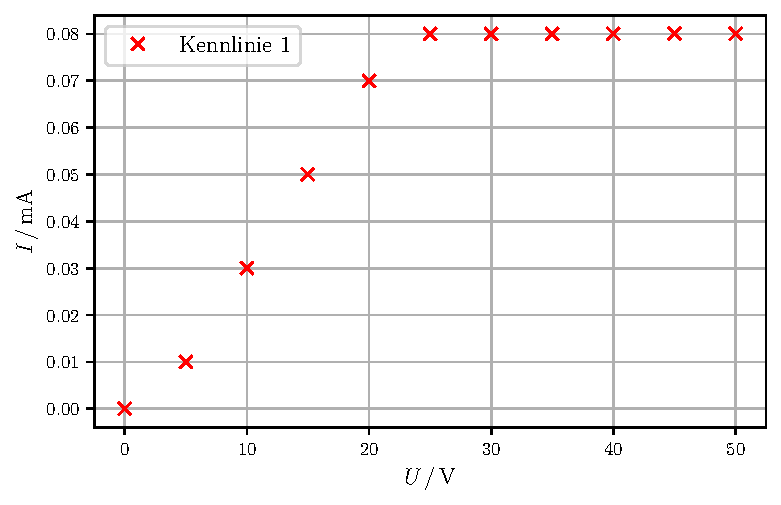
\includegraphics[width=\textwidth]{plot_k1.pdf}
  \caption{Kennlinie 1 mit $I_\text{Heiz} = \qty{2,0}{\ampere}$.}
  \label{fig:k1}
  \end{subfigure}\hfill
  \begin{subfigure}{0.49\columnwidth}
  \centering
  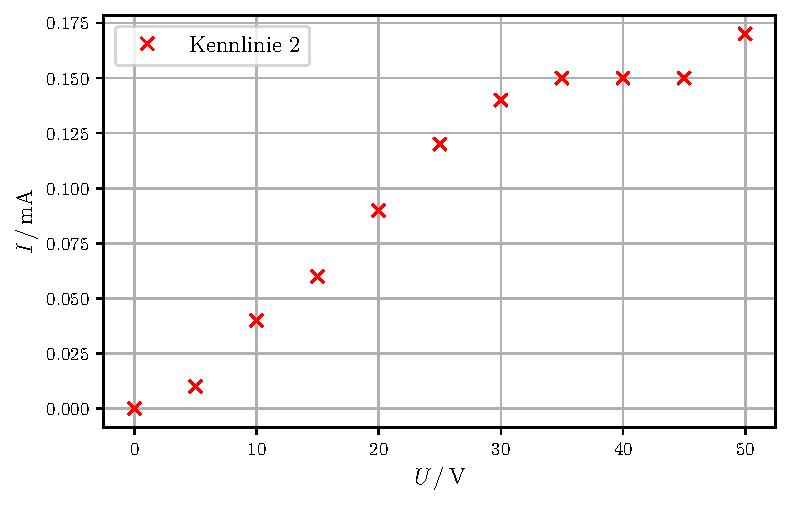
\includegraphics[width=\textwidth]{plot_k2.pdf}
  \caption{Kennlinie 2 mit $I_\text{Heiz} = \qty{2,1}{\ampere}$.}
  \label{fig:k2}
  \end{subfigure}
  
  \medskip
  
  \begin{subfigure}{0.49\columnwidth}
  \centering
  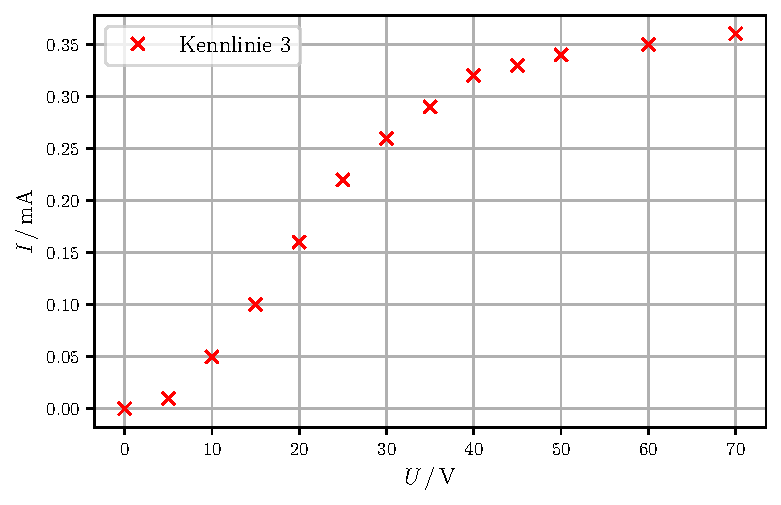
\includegraphics[width=\textwidth]{plot_k3.pdf}
  \caption{Kennlinie 3 mit $I_\text{Heiz} = \qty{2,2}{\ampere}$.}
  \label{fig:k3}
  \end{subfigure}\hfill
  \begin{subfigure}{0.49\columnwidth}
  \centering
  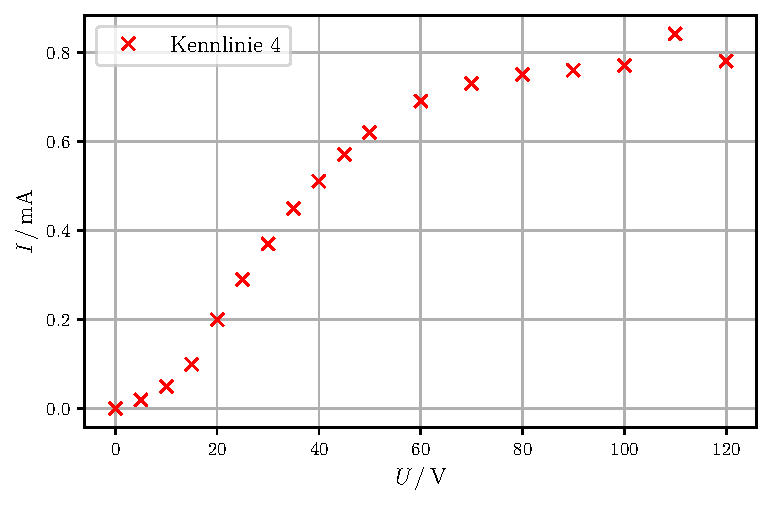
\includegraphics[width=\textwidth]{plot_k4.pdf}
  \caption{Kennlinie 4 mit $I_\text{Heiz} = \qty{2,3}{\ampere}$.}
  \label{fig:k4}
  \end{subfigure}
  
  \medskip
  
  \begin{subfigure}{0.49\columnwidth}
  \centering
  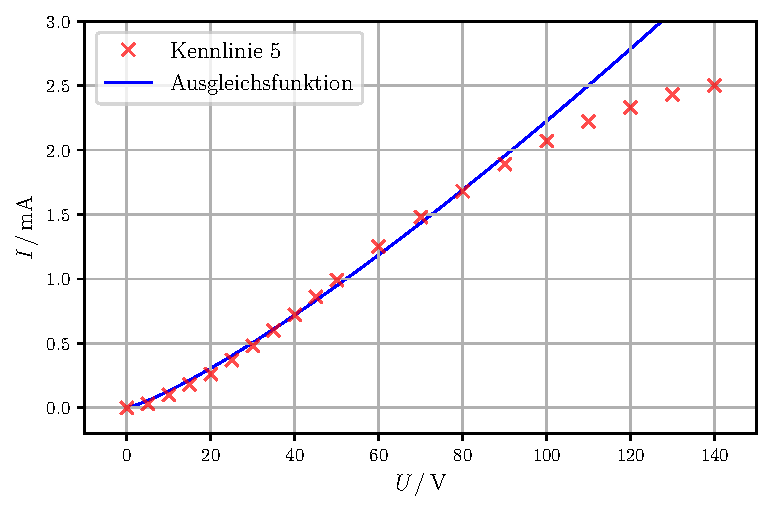
\includegraphics[width=\textwidth]{plot_k5.pdf}
  \caption{Kennlinie 5 mit $I_\text{Heiz} = \qty{2,4}{\ampere}$.}
  \label{fig:k5}
  \end{subfigure}
  
  \caption{Die fünf Kennlinien mit den jeweils angelegten Heiztrömen.}
  \label{fig:k}
\end{figure}

Der Sättigungstrom wird an der Asymptote abgelesen beziehungsweise wie in \autoref{fig:k5} 
mithilfe des Wendepunktes berechnet.
\begin{align*}
  \text{Kennlinie 1} : \quad I_\text{S} &= \qty{0,12}{\milli\ampere} \\
  \text{Kennlinie 2} : \quad I_\text{S} &= \qty{0,27}{\milli\ampere} \\
  \text{Kennlinie 3} : \quad I_\text{S} &= \qty{0,60}{\milli\ampere} \\
  \text{Kennlinie 4} : \quad I_\text{S} &= \qty{1,25}{\milli\ampere} \\
  \text{Kennlinie 5} : \quad I_\text{S} &= \qty{2,10}{\milli\ampere}
\end{align*}

\subsection{Raumladungsgesetz}

Um die Gültigkeit des Raumladungsgesetzes zu überprüfen wird bei der Kennlinie mit
dem höchsten Heizstrom eine Ausgleichsrechung mithilfe des Langmuir-Schottkyschen
Raumladungsgesetzes nach \autoref{eq:lsr} durchgeführt. 
Dabei wird unter anderem der Exponent als freier Parameter gewählt.
\begin{equation*}
  I= \frac{4}{9} \varepsilon_{0} \sqrt{\frac{2 e_{0}}{m_{0}}} \cdot \frac{U^{b}}{a^2}
\end{equation*}
Die Konstanten werden nach \cite{constants} eingesetzt, die dadurch bestimmten Parameter ergeben sich zu
\begin{align*}
  a &= (\num{-49.826(2.123)}) \cdot 10^{-3} \\
  b &= (\num{1.467(0.020)}) \, . 
\end{align*}
Die sich so ergebende Funktion wird in \autoref{fig:k5} eingezeichnet.

\subsection{Anlaufstromgebiet}

In der Tabelle sind die Messwerte des Anlaufstromgebietes eingetragen. Dabei wurde
eine Heizspannung von $I_{\text{Heiz}} = \qty{2.4}{\ampere}$ gewählt.
\begin{table}
  \centering
  \caption{Messwerte des Anlaufstroms.}
  \label{tab:anlaufstrom}
  \begin{tabular}{c c}
    \toprule
    $U \mathbin{/} \unit{\volt}$ &
    $I \mathbin{/} \unit{\milli\ampere}$ \\
    \midrule
    0,00 & 7,0000 \\
    0,10 & 8,1000 \\
    0,20 & 4,6500 \\
    0,30 & 2,5000 \\
    0,40 & 1,2000 \\
    0,50 & 0,4500 \\
    0,60 & 0,4000 \\
    0,70 & 0,2000 \\
    0,80 & 0,0600 \\
    0,90 & 0,0230 \\
    0,96 & 0,0005 \\
    \bottomrule
  \end{tabular}
\end{table}

Die Messwerte werden in ein Diagramm eingetragen und eine Ausgleichsrechung nach \autoref{eq:anlaufstromgebiet}
\begin{equation}
  I=a \cdot \exp \left(\frac{-e_{0} U}{k_{\text{B}} \cdot b}\right)
\end{equation}
durchgeführt. Mit den eingesetzten Konstanten ergeben sich die Parameter zu
\begin{align*}
  a &= \qty{13.228(0.240)}{\nano\ampere} \, , \\
  b &= \qty{2131(70)}{\kelvin} \, . 
\end{align*}
Dabei entspricht der Parameter $b$ der gesuchten Temperatur $T = \qty{3079(568)}{\kelvin}$ .

\begin{figure}
  \centering
  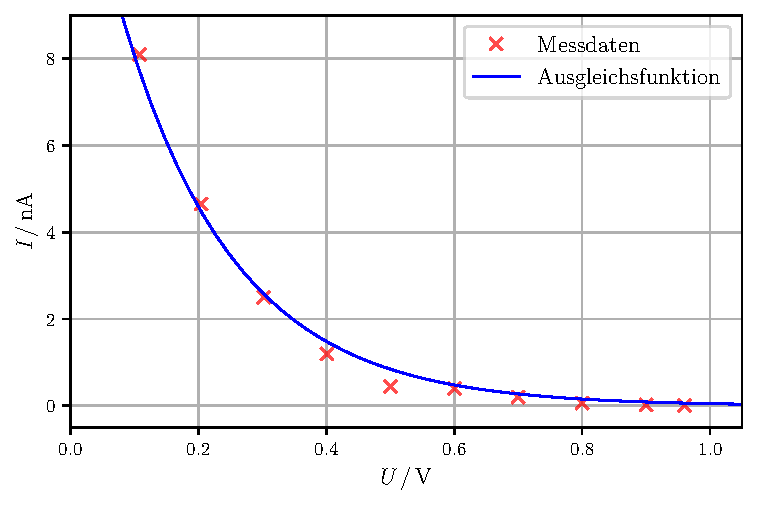
\includegraphics[width=0.8\textwidth]{plot6.pdf}
  \caption{Das Anlaufstromgebiet bei einem Heizstrom von $I_\text{Heiz} = \qty{2,5}{\ampere}$.}
  \label{fig:anlaufstrom}
\end{figure}

\subsection{Kathodentemperatur}

Die Kathodentemperaturen der verschiedenen Kennlinien werden durch eine Betrachtung der Leistungsbilanz bestimmt.
Die zugeführte Leistung beträgt
\begin{equation*}
  N_{\text{zu}}=U_{\text{Heiz}} I_{\text{Heiz}} \, .
\end{equation*}
Diese wird über Wärmestrahlung und Wärmeleitung abgegeben. 
Die Wärmeleitung der Fadenhalterung beträgt $N_{\text{WL}} = \qty{1}{\watt}$. 
Die Srahlungsleistung ergibt sich nach dem Stefan-Boltzmannschen Gesetz zu
\begin{equation*}
  N_{\mathrm{W}}=f \eta \sigma T^{4} \, ,
\end{equation*}
hierbei ist $\sigma=5,7 \cdot 10^{-12} \frac{\mathrm{W}}{\mathrm{cm}^{2} \mathrm{K}^{4}}$ die Stefan-Boltzmannsche Strahlungskonstante, 
$f=$ $0,32 \mathrm{cm}^{2}$ die Kathodenoberfläche und $\eta=0,28$ der Emissionsgrad der Oberfläche. 
Daraus ergibt sich insgesamt
\begin{align*}
N_{\mathrm{zu}} &=N_{\mathrm{W}}+N_{\mathrm{WL}} \\
\Leftrightarrow \quad U_{\mathrm{Heiz}} I_{\mathrm{Heiz}} &=f \eta \sigma T^{4}+N_{\mathrm{WL}}
\end{align*}
Wird die Gleichung nach der Temperatur $T$ umgeformt lassen sich die verschiedenen Temperaturen bestimmen.